% 10_multiscale.tex -- Part 10, from first principles to the device. Sources: research_monograph/chapters/
% M12_multiscale.tex (fig:mono-ms-chain, tab:mono-ms-transfer, tab:mono-ms-budget, sec:mono-ms-explain, keyresult),
% M08_c10_campaign.tex (shared parameters, tab:mono-c10-models, tab:mono-c10-hyp H-E/H-J, S1-05 and audit A13),
% M05_confinement_theory.tex (quasi-2-D N_c, Kane dispersion), M09_masses_parameters.tex (tab:mono-mass-tcad deck gaps;
% Kane factor 5.7 % 3-D / 2.5 % quasi-2-D), M15_conclusions.tex (inferred item 3: 44 / 50 / 18 %; tab:concl-plausible
% C2-C4, required measurements), 09_mechanisms_rev.tex (C-V flat-band scaling, optical-gap falsifier, V1 law 0.353 eV),
% appendices/MG_corrections.tex (X4, X5, X12); report_latex_full/chapters/04_derivations_electrostatics.tex and
% 02d_provenance.tex (chi = 4.30 eV from Fan2021, composition-mixing estimate); evidence/derived/multiscale_budget.json;
% evidence/CLAIM_SOURCE_MAP.tsv (M007, C014, C018); evidence/FACT_REGISTRY.tsv (FACT-027, 030, 060, 101-103).
% Figure 10_rigid.pdf: tools/fig_10_multiscale.py (presentation redraw of research_monograph/figures/
% mono_threshold_vs_dft; data: b03_gaps_laws.json, evidence/derived/device_facts.json, multiscale_budget.json).
% No amorphous quantity and no ATLAS result from S2 on.
% Note: frame bodies start with a command, never with a brace group (beamer would read a subtitle).
\partslide{Part 10}{From first principles to the device}

% denser slides: footnotesize bullets, local to the frame in which it is called
\providecommand{\tendense}{\setbeamerfont{itemize/enumerate body}{size=\footnotesize}%
  \setbeamerfont{itemize/enumerate subbody}{size=\footnotesize}}
\providecommand{\tenTop}{\vspace{-4mm}}
\providecommand{\tenNc}{N_{\mathrm{c}}}
\providecommand{\tenNv}{N_{\mathrm{v}}}
\providecommand{\tenQf}{Q_{\mathrm{f}}}
\providecommand{\tenC}[1]{{\tiny\color{inkgrey}\,#1}}
% evidence label inside \src lines (same vocabulary as \lab, at the size of the source text)
\providecommand{\tenL}[1]{{\color{inkgrey}[\textsc{\MakeLowercase{#1}}]}}
\providecommand{\tenData}{Data: Prof.\ M.-H.\ Lee's group, NTU; one device per thickness}
% budget chart (slide 2): centre of row #1; \dy is set inside the picture
\providecommand{\tenyc}[1]{{0.2-(#1-0.5)*\dy}}
% TikZ styles of this section (defined outside the frames: beamer frames do not accept # in their body)
\tikzset{tenbox/.style={draw, line width=0.4pt, align=flush center, font=\scriptsize, inner sep=2.2pt,
    minimum height=13mm, text width=#1}, tenbox/.default=2.5cm,
  tenlow/.style={draw, line width=0.4pt, align=flush left, font=\scriptsize, inner sep=2.2pt, minimum height=10.5mm,
    text width=#1},
  tenarr/.style={-{Stealth[length=1.6mm]}, line width=0.5pt}}

% ---------------------------------------------------------------------------------------------------------------------
\begin{frame}[t]{Only band-edge increments reach the device model}
  \tenTop\tendense
  \par{\centering
  \begin{tikzpicture}[node distance=3mm and 5mm]
    % main chain
    \node[tenbox] (dft) {\textbf{First principles}\\PBE, crystalline (001)\\films 0.46--1.96\,nm\\\lab{computed}};
    \node[tenbox=2.3cm, right=of dft] (law) {\textbf{Thickness laws}\\$\dEc$, $\dEg$, $\Delta m^{*}$\\
      fit3 to 0.70--1.96\,nm\\\lab{fitted}};
    \node[tenbox=3.2cm, right=of law] (deck) {\textbf{Device inputs}\\$\chi = 4.3\,\mathrm{eV} - \dEc(t)$\\
      $\Eg = 3.05\,\mathrm{eV} + \dEg(t)$\\$\tenNc$, $\mu$: $m^{*} = 0.208\,\mzero + \Delta m^{*}$};
    \node[tenbox=3.85cm, right=of deck] (atlas) {\textbf{ATLAS drift--diffusion}\\electrons only, Fermi--Dirac\\
      $\Vthcc$, SS, $I_\mathrm{on}$ compared\\with the measured curves};
    \draw[tenarr] (dft) -- (law);
    \draw[tenarr, ntumaroon, line width=0.9pt] (law) -- (deck);
    \draw[tenarr] (deck) -- (atlas);
    % lower row
    \node[tenlow=5.25cm, dashed, below=2mm of dft.south west, anchor=north west] (notx)
      {\textbf{Computed, not transferred}\\absolute PBE gaps; HSE06 ratio $r = 1.06$--1.11\\
       W donated density $2.7\times10^{21}$\cmcu{} (bulk cells)\\
       $\tenNv = 1.6$--$2.7\times10^{21}$\cmcu; Kane factor in $\tenNc$};
    \node[tenlow=3.0cm, below=2mm of deck] (lit)
      {\textbf{Bulk anchors} (literature)\\$\chi = 4.3$\,eV, $\Eg = 3.05$\,eV\sref{Fan2021}\\
       $m^{*} = 0.208\,\mzero$\sref[p.~225102-1]{Stokey2021}};
    \node[tenlow=4.3cm, below=2mm of atlas.south east, anchor=north east] (fit)
      {\textbf{Not from first principles}\\fitted: $\Delta V_0$ ($\tenQf$), $\mu_\infty$, $\ell$, $N_{\mathrm{s}}$,
       $W_{\mathrm{TA}}$\\fitted in model V1, fixed in C10: donors $2.5\times10^{17}$\cmcu\\
       assumed: $\tenNv$, deep and interface traps};
    \draw[tenarr, dashed] (dft.south) -- (dft.south |- notx.north);
    \draw[tenarr] (lit) -- (deck);
    \draw[tenarr] (atlas.south |- fit.north) -- (atlas.south);
  \end{tikzpicture}\par}
  \src{C10 decks: fit3 laws incl.\ the polar 0.695\,nm film (caveat: not in the primary $\dEc$ fit); quasi-2-D
    $\tenNc$ at 2.0\,nm (one subband, $E_2 - E_1 = 0.72$\,eV \tenL{computed}); 4.3\,eV: composition-mixing estimate,
    3.05\,eV: optical gap, both of another sputtered IWO device; $m^{*}$ measured; shared fits ($\tenQf$: front charge;
    $\mu_\infty$, $\ell$: mobility law; $N_{\mathrm{s}}$, $W_{\mathrm{TA}}$: tail density, width). W fully ionised
    \tenL{inferred}. Assumed: $\tHH$ = device thickness; OH-terminated crystalline films stand for the device films;
    traps shift rigidly with $\Ec$.}
  \vspace{-0.5mm}
  \begin{itemize}
    \item Effectively one independent law is transferred: the mass increase follows from $\dEc$ by the Kane
      relation\sref{Kane1957} within 1\,\% at 1.962\,nm (10\,\% at 0.930\,nm) \lab{derived}; $\dEg$ enters only $n_i$;
      6.3 and 13.2\,nm are extrapolated.
  \end{itemize}
  \takeaway{Effectively one first-principles law, $\dEc(t)$ (fitted), and an $\tenNc$ convention carry thickness.}
\end{frame}

% ---------------------------------------------------------------------------------------------------------------------
\begin{frame}[t]{A convention, not the crystal, leads the DFT-related budget}
  \tenTop\tendense
  \par{\centering
  \begin{tikzpicture}[x=1cm,y=1cm,font=\scriptsize]
    % columns: source (0 .. 5.6 cm), value (5.7 .. 8.4 cm), log axis 1 .. 1000 mV (8.6 .. 13.55 cm, 1.65 cm/decade)
    \def\ax{8.6}\def\dec{1.65}\def\dy{0.4}\def\nr{6}%
    % row i: centre at 0.2-(i-0.5)*dy, rule below at 0.2-i*dy; the log axis replaces the last rule
    \def\yb{{0.2-\nr*\dy}}
    % reference band: the three 6.3 nm misses, 230 .. 370 mV; dashed: measured 2.0 -> 13.2 nm step, 579 mV
    \fill[black!10] ({\ax+\dec*log10(230)},0.2) rectangle ({\ax+\dec*log10(370)},\yb);
    \draw[dashed, line width=0.5pt] ({\ax+\dec*log10(579)},0.2) -- ({\ax+\dec*log10(579)},\yb);
    % header
    \node[anchor=west, font=\scriptsize\bfseries] at (0,0.42) {Input choice (2.0\,nm unless stated)};
    \node[anchor=west, font=\scriptsize\bfseries] at (5.7,0.42) {Effect on $\Vthcc$ (mV)};
    % key to the two reference marks, right-aligned above the axis area
    \node[anchor=east, inner sep=1pt] (tenk2) at ({\ax+3*\dec},0.42) {2.0--13.2\,nm step\sref{Januar2026}};
    \draw[dashed, line width=0.5pt] ([xshift=-1.2mm]tenk2.west) -- ++(-4.5mm,0);
    \node[anchor=east, inner sep=1pt] (tenk1) at ([xshift=-7.2mm]tenk2.west) {6.3\,nm misses};
    \fill[black!10] ([xshift=-1.2mm, yshift=-1mm]tenk1.west) rectangle ++(-3.2mm,2mm);
    \draw[line width=0.6pt] (0,0.2) -- ({\ax+3*\dec},0.2);
    % rows
    \foreach \i/\lbl/\val in {
        1/{$\tenNc$ convention: quasi-2-D vs 3-D}/{$+142$ (ATLAS, stage S1)},
        2/{Thickness definition, $\pm0.2$\,nm}/{$\approx\pm40$},
        3/{HSE06 ratio on $\dEc$, $r = 1.06$--1.11}/{$+16$ to $+29$},
        4/{$\dEc$ fit options, 0.273--0.289\,eV}/{$\pm8$},
        5/{Kane factor in 3-D $\tenNc$ ($+5.7$\,\%)}/{1.4 free; 5 with tail},
        6/{Mass fit basis ($\pm3$\,\% in $m^{*}$, 3-D $\tenNc$)}/{1 free; 4 with tail}} {
      \node[anchor=west] at (0,\tenyc{\i}) {\lbl};
      \node[anchor=west] at (5.7,\tenyc{\i}) {\val};
      \draw[rulegrey, line width=0.3pt] (0,{0.2-\i*\dy}) -- (\ax,{0.2-\i*\dy});
      \ifnum\i<\nr \draw[rulegrey, line width=0.3pt] (\ax,{0.2-\i*\dy}) -- ({\ax+3*\dec},{0.2-\i*\dy});\fi
    }
    % markers (values: evidence/derived/multiscale_budget.json; M12 tab:mono-ms-budget)
    \fill[ntumaroon] ({\ax+\dec*log10(142)},\tenyc{1}) circle (0.075);
    \fill ({\ax+\dec*log10(40.4)},\tenyc{2}) circle (0.06);
    \draw[line width=1.6pt] ({\ax+\dec*log10(16.4)},\tenyc{3}) -- ({\ax+\dec*log10(29.3)},\tenyc{3});
    \fill ({\ax+\dec*log10(7.65)},\tenyc{4}) circle (0.06);
    \draw[line width=0.5pt] ({\ax+\dec*log10(1.43)},\tenyc{5}) -- ({\ax+\dec*log10(5.02)},\tenyc{5});
    \draw[fill=white, line width=0.5pt] ({\ax+\dec*log10(1.43)},\tenyc{5}) circle (0.06);
    \fill ({\ax+\dec*log10(5.02)},\tenyc{5}) circle (0.06);
    \draw[line width=0.5pt] ({\ax+\dec*log10(1.15)},\tenyc{6}) -- ({\ax+\dec*log10(4.01)},\tenyc{6});
    \draw[fill=white, line width=0.5pt] ({\ax+\dec*log10(1.15)},\tenyc{6}) circle (0.06);
    \fill ({\ax+\dec*log10(4.01)},\tenyc{6}) circle (0.06);
    % log axis
    \draw[line width=0.5pt] (\ax,\yb) -- ({\ax+3*\dec},\yb);
    \foreach \e/\t in {0/1,1/10,2/100,3/1000} {
      \draw ({\ax+\e*\dec},\yb) -- ({\ax+\e*\dec},{0.2-\nr*\dy+0.08});
      \node[anchor=north, inner sep=1.5pt] at ({\ax+\e*\dec},\yb) {\t};
    }
    \foreach \e in {0,1,2} {\foreach \m in {2,3,4,5,6,7,8,9} {
      \draw ({\ax+\e*\dec+\dec*log10(\m)},\yb) -- ({\ax+\e*\dec+\dec*log10(\m)},{0.2-\nr*\dy+0.04});}}
    \node[anchor=north] at ({\ax+1.5*\dec},{0.2-\nr*\dy-0.28}) {$|\Delta\Vthcc|$ (mV, log scale)};
  \end{tikzpicture}\par}
  \src{Row 1: ATLAS run S1-05, seen before register revision 2 \tenL{computed}; rows 2--6 \tenL{derived} (laws, audit
    A13); rows 5--6 in the 3-D $\tenNc$ form; open: free carriers, filled: with tail filling. Band: 0.23--0.37\,V;
    dashed: measured 2.0--13.2\,nm step, 0.579\,V. Crystalline vs amorphous: unknown, H-K sealed (Part 11). \tenData.}
  \vspace{-0.5mm}
  \begin{itemize}
    \item In the model, $\dEc$ shifts $\Vthcc$ one-to-one by construction (traps move with $\Ec$; test H-E sealed); mass
      and $\tenNc$ act through the statistics, amplified about 3.5 times by the 40\,meV tail (registered audit A13;
      Part 4).
  \end{itemize}
  \takeaway{Ranking: $\tenNc$ convention, thickness definition, functional; the rest is minor.}
\end{frame}

% ---------------------------------------------------------------------------------------------------------------------
\begin{frame}[t]{Rigid $\dEc$ gives 44\,\% of the 2.0--13.2\,nm step, 0.2\,V off at 6.3\,nm}
  \tenTop\tendense
  \begin{columns}[T,onlytextwidth]
    \begin{column}{0.43\textwidth}
      \centering
      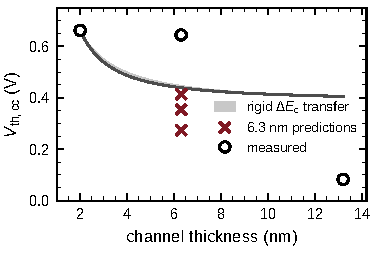
\includegraphics[width=\linewidth]{10_rigid}
      \raggedright
      \src{Measured $\Vthcc$ (circles) against $\Vthcc(2.0) + [\dEc(t) - \dEc(2.0)]/q$ (band: four fit options; line:
        two-point fit). Crosses: failed 6.3\,nm predictions (C014). Rigid 1:1 transfer, not a model run \tenL{derived}.
        \tenData.}
    \end{column}
    \begin{column}{0.54\textwidth}
      \begingroup\scriptsize
      \setlength{\tabcolsep}{6pt}
      \renewcommand{\arraystretch}{0.98}
      \begin{tabular}{@{}l c c@{}}
        \toprule
        $\Delta\Vthcc$ (V) & rigid $\dEc$ & measured\sref{Januar2026} \\
        \midrule
        2.0 $\to$ 13.2\,nm & $-0.257$ & $-0.579$ \\
        2.0 $\to$ 6.3\,nm & $-0.21$ to $-0.22$ & $-0.018$ \\
        \midrule
        6.3\,nm misses & \multicolumn{2}{c}{$-0.29$, $-0.37$, $-0.23$ \lab{falsified}} \\
        \bottomrule
      \end{tabular}\par\endgroup
      \src{Rigid: fit-option spread below 2\,meV (2.0--13.2\,nm). Misses: model V1 run 0014; model V2 P, E, run 0060
        (Part 4). Claims M007 \tenL{derived}, C018. Causes: Part 12.}
      \begin{itemize}
        \item 2.0--13.2\,nm step: the rigid shift is 44\,\% of it \lab{derived}; other model inputs partly cancel
          it (audit A13 forecast $\approx$18\,\%; earlier calibration $\approx$50\,\%).
        \item 2.0 to 6.3\,nm: the rigid shift puts 6.3\,nm $\approx$0.2\,V too low, like all three misses. No cause
          assigned: the device acts as if much thinner, or as if charge raised $\Vthcc$ by 0.2\,V.
        \item Model V2 vs model V1, like with like: this work's DFT laws shrink the miss by only $\approx$0.04\,V
          \lab{computed}.
      \end{itemize}
    \end{column}
  \end{columns}
  \takeaway{Confinement alone does not carry the 2.0--13.2\,nm step \lab{inferred}.}
\end{frame}

% ---------------------------------------------------------------------------------------------------------------------
\begin{frame}[t]{Three probes and device statistics can separate the inputs}
  \tenTop\tendense
  \begin{itemize}
    \item In transfer curves, gate work function, bulk affinity, a uniform fixed charge and $\dEc$ act as one number
      per film \lab{derived}; a shared $\Delta V_0$ for three films (registered campaign, sealed) is the first test
      the computed inputs can fail.
  \end{itemize}
  \vspace{0.5mm}
  \begingroup\scriptsize
  \setlength{\tabcolsep}{4pt}
  \renewcommand{\arraystretch}{1.1}
  \begin{tabularx}{\textwidth}{@{}>{\raggedright\arraybackslash}p{3.2cm}>{\raggedright\arraybackslash}p{4.0cm}
      >{\raggedright\arraybackslash}X@{}}
    \toprule
    Measurement against $t$ & What it separates & Value or falsifier at stake \\
    \midrule
    C--V flat band $V_{\mathrm{FB}}(t)$ & charges by their scaling: front sheet $t^0$, volume $t$ and $t^2$, back sheet
      $t/\varepsilon_s$ &
      donor or positive-charge step at 13.2\,nm: falsified if $V_{\mathrm{FB}}(t)$ is flat within 50\,mV \\
      \addlinespace[1pt]
    Optical gap & confinement, a band-edge property, from charge &
      deck gaps 3.38, 3.12, 3.08\,eV at 2.0, 6.3, 13.2\,nm; confinement falsified if the 2.0--13.2\,nm shift is
      below 0.1\,eV \\ \addlinespace[1pt]
    Photoemission offsets (UPS, IPES), Kelvin probe & $\chi(t)$ and work function directly: $\dEc$ apart from
      $\tenQf$ &
      this work's DFT: $\dEc(2.0) = 0.273$--0.289\,eV over fit options (model V1 law, fitted to published slab DFT:
      0.353\,eV); $\times1.06$--1.11 with HSE06 \\ \addlinespace[1pt]
    $\ge 10$ devices per thickness, one run, dual sweeps & device spread from a film property &
      device-specific 6.3\,nm offset: falsified if the mean is $\ge 0.2$\,V off a smooth law with
      $\sigma(\Vth) < 0.1$\,V \\
    \bottomrule
  \end{tabularx}\par\endgroup
  \src{Right column: the monograph's plausible-mechanism conjectures with their falsifiers; campaign
    C10; claim C018. Deck gaps: PBE increments on the 3.05\,eV optical anchor (first slide of this part) \tenL{derived};
    $\dEc$: fit3, C10 decks. $\tenQf$: front fixed charge; $\varepsilon_s$:
    channel permittivity. None of these measurements exists yet for the present films.}
  \takeaway{Band-edge and charge probes can isolate the shift; replicates test the 6.3\,nm offset.}
\end{frame}
